\section{Results}\label{sec:results}

All numbers in this section come from the one-shot test runs.

% generated by scripts/12_paper_tables.py from results/03_test3.json (v3 one-shot test)
\begin{table}[t]\centering\scriptsize
\caption{One-shot test results on the simulated regimes. RMSE ($\times10^{-3}$) of \odrift{}, of its configuration without offset shrinkage (v1) and of the best tuned baseline in the cell; ratio of \odrift{} to that baseline ($^{*}$: paired 95\% interval of the RMSE difference excludes 0); coverage of the nominal 95\% heterogeneity-adjusted interval. 300 episodes $\times$ 4 policies per cell.}
\label{tab:main}
\begin{tabular}{@{}lccrrlrrr@{}}\toprule
Regime & Int. & Misspec. & \odrift{} & v1 & Best tuned baseline & RMSE & Ratio & Cov. \\\midrule
S0 & 0 & 0.5 & 5.4 & 5.4 & Min-var DR & 5.1 & 1.05$^{*}$ & 0.93 \\
S1 & 0.5 & 0.5 & 5.5 & 5.5 & COPE & 5.5 & 1.00 & 0.95 \\
S1 & 2 & 0.5 & 8.0 & 8.0 & COPE & 7.8 & 1.02 & 0.93 \\
S2 & 0 & 0.5 & 5.1 & 5.1 & Balanced DR & 4.7 & 1.07$^{*}$ & 0.95 \\
S3a & 0.25 & 0.5 & 6.4 & 6.5 & Monitor-select DR & 7.0 & 0.93$^{*}$ & 0.89 \\
S3a & 1 & 0.5 & 9.8 & 6.5 & Monitor-select DR & 7.0 & 1.40$^{*}$ & 0.83 \\
S3b & 0.25 & 0.5 & 10.9 & 10.8 & Time-DR & 8.5 & 1.28$^{*}$ & 0.63 \\
S3b & 1 & 0.5 & 26.6 & 18.4 & Time-DR & 8.8 & 3.02$^{*}$ & 0.27 \\
S4 & 0.25 & 0.5 & 7.5 & 8.0 & Balanced DR & 8.6 & 0.86$^{*}$ & 0.95 \\
S4 & 1 & 0.5 & 14.1 & 14.8 & T-recent DR & 21.7 & 0.65$^{*}$ & 0.78 \\
S5 & 0.5 & 0.5 & 21.5 & 20.9 & Decay DR & 20.4 & 1.05$^{*}$ & 0.34 \\
S5 & 1 & 0.5 & 34.7 & 28.9 & SLOPE & 36.0 & 0.96 & 0.22 \\
S6 & 0 & 0.5 & 5.9 & 5.9 & Balanced DR & 5.3 & 1.13$^{*}$ & 0.94 \\
S7 & 0 & 0.5 & 7.4 & 7.4 & Min-var DR & 4.9 & 1.52$^{*}$ & 0.94 \\
S8 & 0.5 & 0.5 & 6.7 & 6.7 & Monitor-select DR & 7.0 & 0.96 & 0.88 \\
S8 & 1 & 0.5 & 6.9 & 6.8 & Monitor-select DR & 7.0 & 0.98 & 0.86 \\
S8b & 1 & 0.5 & 6.7 & 6.7 & Monitor-select DR & 7.0 & 0.96 & 0.89 \\
S0 & 0 & 3 & 4.9 & 4.9 & Pooled DR & 4.5 & 1.08$^{*}$ & 0.95 \\
S2 & 0 & 3 & 5.0 & 5.0 & Balanced DR & 4.6 & 1.08$^{*}$ & 0.95 \\
S3a & 1 & 3 & 6.5 & 6.7 & Monitor-select DR & 6.7 & 0.98 & 0.86 \\
S4 & 1 & 3 & 17.9 & 25.7 & TB-decay DR & 22.0 & 0.81$^{*}$ & 0.70 \\
S5 & 1 & 3 & 23.3 & 26.2 & Monitor-select DR & 29.2 & 0.80$^{*}$ & 0.33 \\
S8 & 1 & 3 & 6.6 & 6.7 & Monitor-select DR & 6.7 & 0.99 & 0.86 \\
\bottomrule\end{tabular}\end{table}


\paragraph{Simulated regimes.}
\Cref{tab:main} compares \odrift{} with the best tuned baseline in each cell, which differs
from cell to cell. Without reward drift (S0--S2) \odrift{} is within
7\% of the best baseline; the small losses in S0 and S2 are the price of estimating segment
models that turn out to be unnecessary. Under abrupt and mixed reward drift it wins: by 7\% in
S3a at the lower intensity and by 14\% and 35\% in S4, with paired intervals that exclude zero.
In S4 the best baseline changes from balanced DR to transported recent-window DR as the
intensity grows, while \odrift{} is best in both. The misspecification-3 cells of S3a, S4,
S5 and S8 are also won or tied (ratios 0.80--0.99).

It loses in four places. Gradual drift (S3b) violates the piecewise assumption and favours
the trend-modelling time-aware DR (1.28, 3.02).
Under abrupt drift at the higher intensity (S3a, intensity 1) \odrift{} loses to
monitor-select (1.40); here the v1 configuration without offset shrinkage would have won
(6.5 vs.\ 7.0), so the shrinkage tuned on development data under-corrects large drift.
The same holds for S5. In S7 (support loss) the estimator correctly puts no weight on
support-deficient windows, but loses accuracy against min-variance pooling (1.52). The
heterogeneity-inflated interval undercovers whenever bias remains, most severely in S5 and
S3b (0.22--0.63); the certified sample-split interval covers in every regime but is about
18 times wider.

\begin{figure}[t]\centering
\begin{minipage}[c]{0.46\linewidth}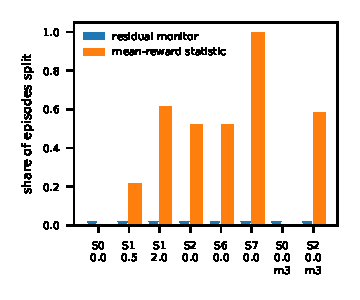
\includegraphics[width=\linewidth]{figures/fig_splits.pdf}\end{minipage}\hfill
\begin{minipage}[c]{0.5\linewidth}
\caption{Share of test episodes in which the history is split into more than one segment, in
regimes without reward drift, for the residual monitor (zero in every cell) and for the
mean-reward statistic (same segmentation procedure and threshold grid).}
\label{fig:splits}
\end{minipage}
\end{figure}

\paragraph{Does the mechanism matter?}
Two pre-registered checks address this (right half of \cref{tab:main}, \cref{fig:splits}).
Against tuned COPE, which groups windows by mean reward, \odrift{} has lower RMSE in all 15
reward-drift cells (ratios 0.19--0.93, intervals excluding zero) and ties it in S0--S2; COPE is
better only in S6 and S7 (1.07, 1.30), with faulty propensities or lost support. The
grouping ablation keeps the whole \odrift{} pipeline and replaces only the monitor statistic by
the mean reward. The residual monitor never splits the history when the
reward is stable (S0--S2, and S6--S7), as \cref{prop:invariance} predicts, whereas the mean-reward
statistic splits 22--61\% of S1 histories under context drift, 52\% of S2 histories under
logger switches and every S7 history. These spurious splits shrink the reference segment and
cost 7--13\% RMSE in S1 and S2. Under reward drift the blind grouping is never better and is worse
in most cells (up to $2.35\times$), mainly because it misses abrupt
changes: in S3a at the lower intensity it detects the change in 29\% of episodes, against 100\%
for the monitor.

% generated by scripts/12_paper_tables.py from results/03_obd3.json (v3 one-shot, Open Bandit)
\begin{table}[t]\centering\scriptsize
\caption{One-shot test on semi-synthetic Open Bandit data (200 episodes per cell). RMSE and mean error (bias) $\times10^{-3}$; v1 is \odrift{} without offset shrinkage; monitor-select uses the same segmentation without reuse. Ratio as in Table~\ref{tab:main}.}
\label{tab:obd}
\begin{tabular}{@{}lcrrrrlrr@{}}\toprule
Regime & Int. & \odrift{} & Bias & v1 & Monitor-select & Best tuned baseline & RMSE & Ratio \\\midrule
S0 & 0 & 3.2 & +0.4 & 3.2 & 3.3 & COPE & 3.1 & 1.03 \\
S2 & 0 & 2.8 & +0.3 & 2.8 & 3.6 & COPE & 2.8 & 1.00 \\
S3a & 0.5 & 15.7 & +13.6 & 7.5 & 4.7 & Monitor-select DR & 4.7 & 3.33$^{*}$ \\
S3a & 1 & 36.4 & +32.2 & 10.0 & 4.7 & Monitor-select DR & 4.7 & 7.74$^{*}$ \\
S4 & 0.5 & 32.0 & +28.1 & 21.1 & 13.6 & Time-DR & 10.2 & 3.14$^{*}$ \\
S4 & 1 & 73.8 & +66.4 & 31.8 & 13.5 & T-recent DR & 10.7 & 6.87$^{*}$ \\
S5 & 1 & 75.4 & +68.0 & 58.5 & 27.3 & Reg.-DR (Liu) & 20.7 & 3.63$^{*}$ \\
\bottomrule\end{tabular}\end{table}


\paragraph{Open Bandit: where drift-corrected reuse fails.}
\Cref{tab:obd} shows the pre-registered robustness test on Open Bandit. Without reward drift
\odrift{} matches the best baseline, but under reward drift it is 3.1--7.7 times worse, and
almost all of its error is bias ($+14$ to $+68\times10^{-3}$). The monitor is not the cause: it
finds the change in every S3a episode, and monitor-select, which uses the same segmentation
without reuse, is the best method in S3a and within a factor of 1.4 of the best in S4. The failure lies in the correction. The base
reward is quadratic, the reward models linear (the basis rule chose linear features in every
episode), and the drift three times the standard deviation of the base logit, so the offsets
$\delta_j$ absorb model error as well as drift and the corrected segments carry a bias the
anchor cannot observe. Offset shrinkage
makes this worse (S3a, intensity 1: 36.4 vs.\ 10.0 without shrinkage). Robustness criteria R1--R2
therefore fail; the other ten pre-registered criteria (C1--C5, N1--N2) pass.

% generated by scripts/13_revisions_table.py (dev episodes only; post-hoc revisions, never tested)
\begin{table}[t]\centering\scriptsize
\caption{Post-hoc revisions on development data (52 matched episodes per cell). RMSE of each version divided by the RMSE of the best tuned baseline (shown, $\times10^{-3}$). v1: no offset shrinkage; v3: shrinkage 0.25 (the tested version); v4: reuse gate at $z=1.96$; v5: rolling-origin back-test, with the share of episodes in which it chose full reuse, shrunk reuse or no reuse.}
\label{tab:revisions}
\begin{tabular}{@{}lccrrrrrrrr@{}}\toprule
 & & & & \multicolumn{4}{c}{RMSE ratio} & \multicolumn{3}{c}{v5 choice} \\\cmidrule(lr){5-8}\cmidrule(l){9-11}
Reg. & Int. & Mis. & Best & v1 & v3 & v4 & v5 & Reuse & Shrink & None \\\midrule
S0 & 0 & 0.5 & 6.3 & 1.00 & 1.00 & 1.00 & 1.01 & 0.50 & 0.00 & 0.50 \\
S1 & 1 & 0.5 & 7.0 & 0.96 & 0.96 & 0.96 & 1.42 & 0.69 & 0.00 & 0.31 \\
S2 & 0 & 0.5 & 5.5 & 0.99 & 0.99 & 0.99 & 1.23 & 0.58 & 0.00 & 0.42 \\
S3a & 0.5 & 0.5 & 7.7 & 0.89 & 0.86 & 0.89 & 0.95 & 0.33 & 0.27 & 0.40 \\
S3b & 0.5 & 0.5 & 8.5 & 1.02 & 1.09 & 1.02 & 0.99 & 0.31 & 0.27 & 0.42 \\
S4 & 0.5 & 0.5 & 11.9 & 0.89 & 0.71 & 1.32 & 1.53 & 0.29 & 0.38 & 0.33 \\
S0 & 0 & 3 & 5.1 & 1.00 & 1.00 & 1.00 & 0.99 & 0.46 & 0.00 & 0.54 \\
S3a & 0.5 & 3 & 7.1 & 0.93 & 0.85 & 0.94 & 0.97 & 0.27 & 0.33 & 0.40 \\
S4 & 0.5 & 3 & 10.9 & 1.32 & 0.94 & 1.61 & 1.79 & 0.35 & 0.31 & 0.35 \\
\bottomrule\end{tabular}\end{table}


\paragraph{Can reuse be validated on the data at hand? (post-hoc).}
After this test we tried, on development data only, two ways to decide per episode whether to
reuse corrected segments (\cref{tab:revisions}). A gate (v4) that drops a segment whose estimate
differs from the reference (reference segment plus anchor) at the 5\% level removes the bias but
raises the variance, and loses in S4 ($1.32\times$ the best baseline) and in S4 at
misspecification 3 ($1.61\times$). A rolling-origin back-test (v5) treats the newest
history window as a pseudo-target and chooses among full reuse, shrunk reuse and no reuse; it rejects reuse in 31--54\% of episodes without reward drift, where reuse is exactly
right, and is worse than the best fixed version in six of nine cells (up to
$2.1\times$) and tied in a seventh. Neither was tested. Both fail for the reason given in \cref{sec:setting}: a 1{,}000-record anchor gives a DR
RMSE of $42\times10^{-3}$ (a 4{,}000-record window about half), while the decisive reuse bias is
about $10\times10^{-3}$.

\paragraph{How large must the anchor be? (post-hoc).}
With anchors of 100, 1{,}000 and 10{,}000 records (eight cells, frozen v3), anchor-only DR
follows $1/\sqrt{n_T}$ (RMSE $153$, $42$, $12\times10^{-3}$) while \odrift{} hardly moves (S4:
$14.2$, $14.1$, $11.1$; no anchor: $68.5$): segmentation uses history, and 100 records identify the
reference. Under gradual or seasonal drift (S3b, S5), however, the large anchor alone wins
($11.9$ vs.\ $23.5$, $29.3$), since reuse bias does not shrink with $n_T$.
